\newcommand{\ReportSection}[4]{%
    \section{#1}  % First argument is the section title
    \label{sec:#1}
    #2
    \subsection{Reporte}
    \label{subsec:report#1}
    #3
    \subsection{Competencias}
    \label{subsec:competences#1}
    #4
}
\chapter{Reporte de tareas}
\label{ch:taskReport}

En este capítulo se describirá las tareas realizadas en cada parte de las prácticas, lo que se ha aprendido de ellas y como complementan las competencias cursadas en el grado de Ingeniería Aeroespacial de la UCLM.

%\ReportSection{Título Sección}{Intruccion}{Reporte}{Competencias}

\ReportSection
{SoftSkills}{}
{
    Durante esta parte de las prácticas se trabajó con el departamento de recursos humanos, en concreto con Leticia Llamazares y el director del departamento, Pierre Morel.
    Se comenzó por presentar el curso con su cronograma, el personal que nos lo impartiría y lo que se esperaba de nosotros.
    Tras esto, se comenzó a explorar el concepto de Autoconocimiento DISC, que consiste en un test personal capaz de categorizarte según tu personalidad. Con este conocimiento se pretende ser consciente de tus inclinaciones de conducta, así como la de los demás, de forma que te puedas adaptar dependiendo de la situación, facilitando la comunicación.
    
    Además, se realizaron presentaciones de prueba para evaluar y corregir fallos a la hora de expresarse y ganar atención del público.
    
    Finalmente se discutieron técnicas de brainstorming para incentivar la aportación de ideas nuevas, evitar estancamienos y, posteriormente, filtrar los resultados.
    
    Lo aprendido durante este periodo se espera que se ponga en uso en la presentación de proyecto en el cierre de las prácticas.
    
}
{
    Se considera que lo aprendido en este periodo expande las competencias que se pretenden enseñar en la universidad con la asignación de trabajos en grupos y presentaciones, aunque de forma más específica a un sector empresarial, donde mantener un buen ambiente laboral y ser capaz de tratar con desconocidos sin que suponga un impedimento.
}

\ReportSection
{KNX, ETS y Catálogo}{}
{
    Durante esta parte de la formación Francisco Fuentes y Pablo Fernández nos han familiarizado con los productos de la empresa, el protocolo que emplean para comunicarse, KNX, y el software con el que se configuran.
    
    Se comenzó por una explicación del protocolo KNX, un sistema descentralizado desarrollado por \emph{KNX Association}, que permite la transmisión de información y electricidad en un mismo par de cable. Se nos habló sobre sus capacidades, su topología y de sus limitaciones.
    
    Posteriormente se explicaron todas las categorías de productos que ofrece la compañía, profundizando sobre los productos pertenecientes a cada segmento y su funcionamiento.
    
    Se hizo especial énfasis en los sistemas termostatos y de climatización por aire, \emph{FanCoil}.
    
    Por último se trabajó con un equipo de pruebas que emula un sistema real en miniatura y se realizaron prácticas tratando de programar distintos funcionamientos empleando el software ETS.
    
    Las prácticas consistieron en:
    \begin{enumerate}
        \item Accionar elementos de iluminación
        \item Leer elementos de control y vincularlos a los actuadores de la practica anterior.
        \item Configurar un termostato
        \item Usar el resto de prácticas para configurar un sistema FanCoil
    \end{enumerate}
    
}
{
    Esta sección de la formación es especialmente específica a la empresa, sus productos y su forma de operar. Por lo tanto, la conexión con competencias de la universidad se limita a aprender ha adaptarse a los métodos y entornos de desarrollo de una empresa de forma efectiva. Conocimientos de programación y de segmentación y organización de problemas también podrán aplicar.
}

\ReportSection
{Electrónica Básica}{}
{
    En esta sección de las prácticas Verónica Fernández y Carlos Morillo se han encargado de impartir, en primer lugar, aspectos básicos de electrónica como las leyes de Ohm o Kirchhoff y posteriormente circuitos típicos empleados en los dispositivos de Zennio.
    Las lecciones han comenzando siendo teóricas, y una vez afianzados los conocimientos se ha pasado a estudiar los comportamientos de circuitos reales mediante osciloscopio.
    
    Algunos de los circuitos estudiados son:
    \begin{itemize}
        \item Interruptores
        \item Filtros RC
        \item Protecciones contra descargas electromagnéticas
        \item Amplificadores
    \end{itemize}
}
{
    Estas lecciones repasan, amplían y ponen en práctico lo aprendido en las asignaturas de \emph{Física II}, \emph{Electrónica y Automática} y \emph{Electrotecnia}.
}

\ReportSection
{Programación C}{}
{
    Durante este periodo Alfonso Toledo y Esteban García impartieron las bases del lenguaje de programación C. Se comenzó explicando unos programas simples como ejemplo de la sintaxis del lenguaje y posteriormente se explicó el proceso de compilación.
    
    Tras la introducción se comenzó a expandir los conceptos generales como las variables, los operadores, el control de flujo, las funciones y los punteros. Todo ello acompañado de ejercicios prácticos evaluados. \add{cita a ejemplos}.
    
    Con los conceptos básicos asimilados se pasó a explicar funcionalidades más complejas como las estructuras, las constantes, el preprocesador, las librerias, y la memoria dinámica. Tambien acompañados de ejercicios. \add{cita a ejemplos}.
    
    Finalmente se explicaron brevemente las funciones públicas y privadas, así como los punteros a función.
}
{
    Los conceptos adquiridos sobre programación C amplían significativamente las materias dadas en la asignatura de Informática sobre Python y en varias otras sobre MatLab.
}

\ReportSection
{Código limpio y Patrones de diseño}{}
{
    En esta sección Matthew McKay instruyó sobre formas de plantear y estructurar el código de un programa de forma el código resultante sea producido con una mejor calidad y con la capacidad de ser ampliado y probado sin un gasto de recursos significativo.
    
    Algunos de los temas tratados fueron como emplear nomenclaturas significativas, como estructurar funciones para agilizar su empleo, como y cuando comentar código, formas de estructurar un programa globalmente y como plantear pruebas unitarias para comprobar rápidamente si los módulos de un programa funcionan.
}
{
    Aunque los conceptos aprendidos durante estas lecciones no tienen una correspondencia directa con ninguna asignatura, la filosofía impartida sobre como plantear y estructurar código puede ser extrapolada a multitud de casos ingenieriles, haciendo que sean más asequibles, expansibles y seguros.
}

\ReportSection
{Pruebas y Testing}{}
{
    En esta parte Antonio Carrillo explica cómo plantear, diseñar y llevar a cabo pruebas, reportando de forma correcta el procedimiento y resultados.
    
    Se comenzó explicando los principios básicos del testing tras lo que se discutieron distintas tipologías que se pueden emplear dependiendo del caso a estudiar. Posteriormente se explicó el proceso de diseño de pruebas y como gestionarlas de forma segura y sistemática.
    
    El proceso se dividiría en:
    \begin{enumerate}
        \item Planificación y estimaciones
        \item Seguimiento y reportes
        \item Riesgos y pruebas
        \item Gestión de incidencias
    \end{enumerate}
    
    Una vez entendidos los conceptos del testing, se explicó como Zennio aplica esta filosofía en el desarrollo de sus productos para garantizar calidad. Comenzando por el tipo de pruebas que realizan:
    
    \begin{itemize}
        \item Funcionalidad: A nivel de software.
        \item Integración: A ninvel de un sistema completo.
        \item Máximos: A nivel de hardware.
    \end{itemize}
    
    Seguido del flujo de trabajo:
    
    \begin{itemize}
        \item Waterfall
        \item AGILE
    \end{itemize}
    
    Y finalizando con las pruebas específicas que son necesarias por los productos de la empresa.
    
    La última lección en esta parte trató el software EITT, empleado para automatizar el testing de dispositivos que emplean el protocolo KNX.
    
    Todas las lecciones fueron acompañadas de ejercicios basados en casos prácticos en los que se pidió diseñar planes de testeo de algún producto.
}
{
    Los conceptos aprendidos sobre testing encajan con lo aprendido en Ingeniería de la producción sobre control de calidad, y suponen una expansión práctica de la asignatura.
}

\ReportSection
{Software embebido}{}
{
    Durante esta sección de las prácticas Santiago Rodríguez Palma nos explica el flujo de trabajo y las herramientas utilizadas para desarrollar el software para un producto de Zennio.
    
    Se comienza explicando el IDE MCUXpresso que se emplea para crear el código que flasheamos en los microprocesadores.
    
    Seguido, se introduce SVN, un software de control de versiones similar a git con el que la empresa lleva un control de todo su software.
    
    Posteriormente, se realiza una introducción al software embebido de forma genérica.
    Una vez explicados todos los conceptos generales se entra en la organización de código que se realiza en la empresa y en las prácticas que se deben seguir para mantener unos repositorios y control de versiones eficaces.
    
    Por último se enseñan ejemplos de código reales para el producto \emph{InBox 24}y se nos propone realizar fragmentos de código para implementar funcionalidad básica al dispositivo como:
    \begin{itemize}
        \item Encender un led.
        \item Hacer parpadear un led.
        \item Controlar un LED mediante botones.
        \item Controlar LEDS mediante el protocolo KNX.
    \end{itemize}
}
{
    Lo aprendido durante este periodo es una ampliación significativa del temario visto en Informática, Electrónica y Automática y Equipos y Sistemas Confiables. Dando una perspectiva a como se aplica lo aprendido en clase en un entorno empresarial serio y a una mayor escala.
}

\ReportSection{Presentación}{}
{
A lo largo de la práctica, sus 7 miembros fueron reuniendose de forma semanal para coordinar y desarrollar un producto apto para el mercado de Zennio.

Tras una lluvia de ideas y proceso de eliminación se optó por realizar un dispositivo capaz de monitorizar automatizar el regado de un jardín. Y mediante una discusión de capacidades y preferencias se seleccionó el papel de cada individuo.

El producto final se nombró MaxGardenBOX siguiendo la estrategia de nomenclatura de otros productos como ALLinBOX o MAXinBOX. Un actuador multifunción de montura en rail capaz de tomar lecturas de temperatura y humedad y accionar válvular para regado.

\begin{figure}[H]
    \centering
    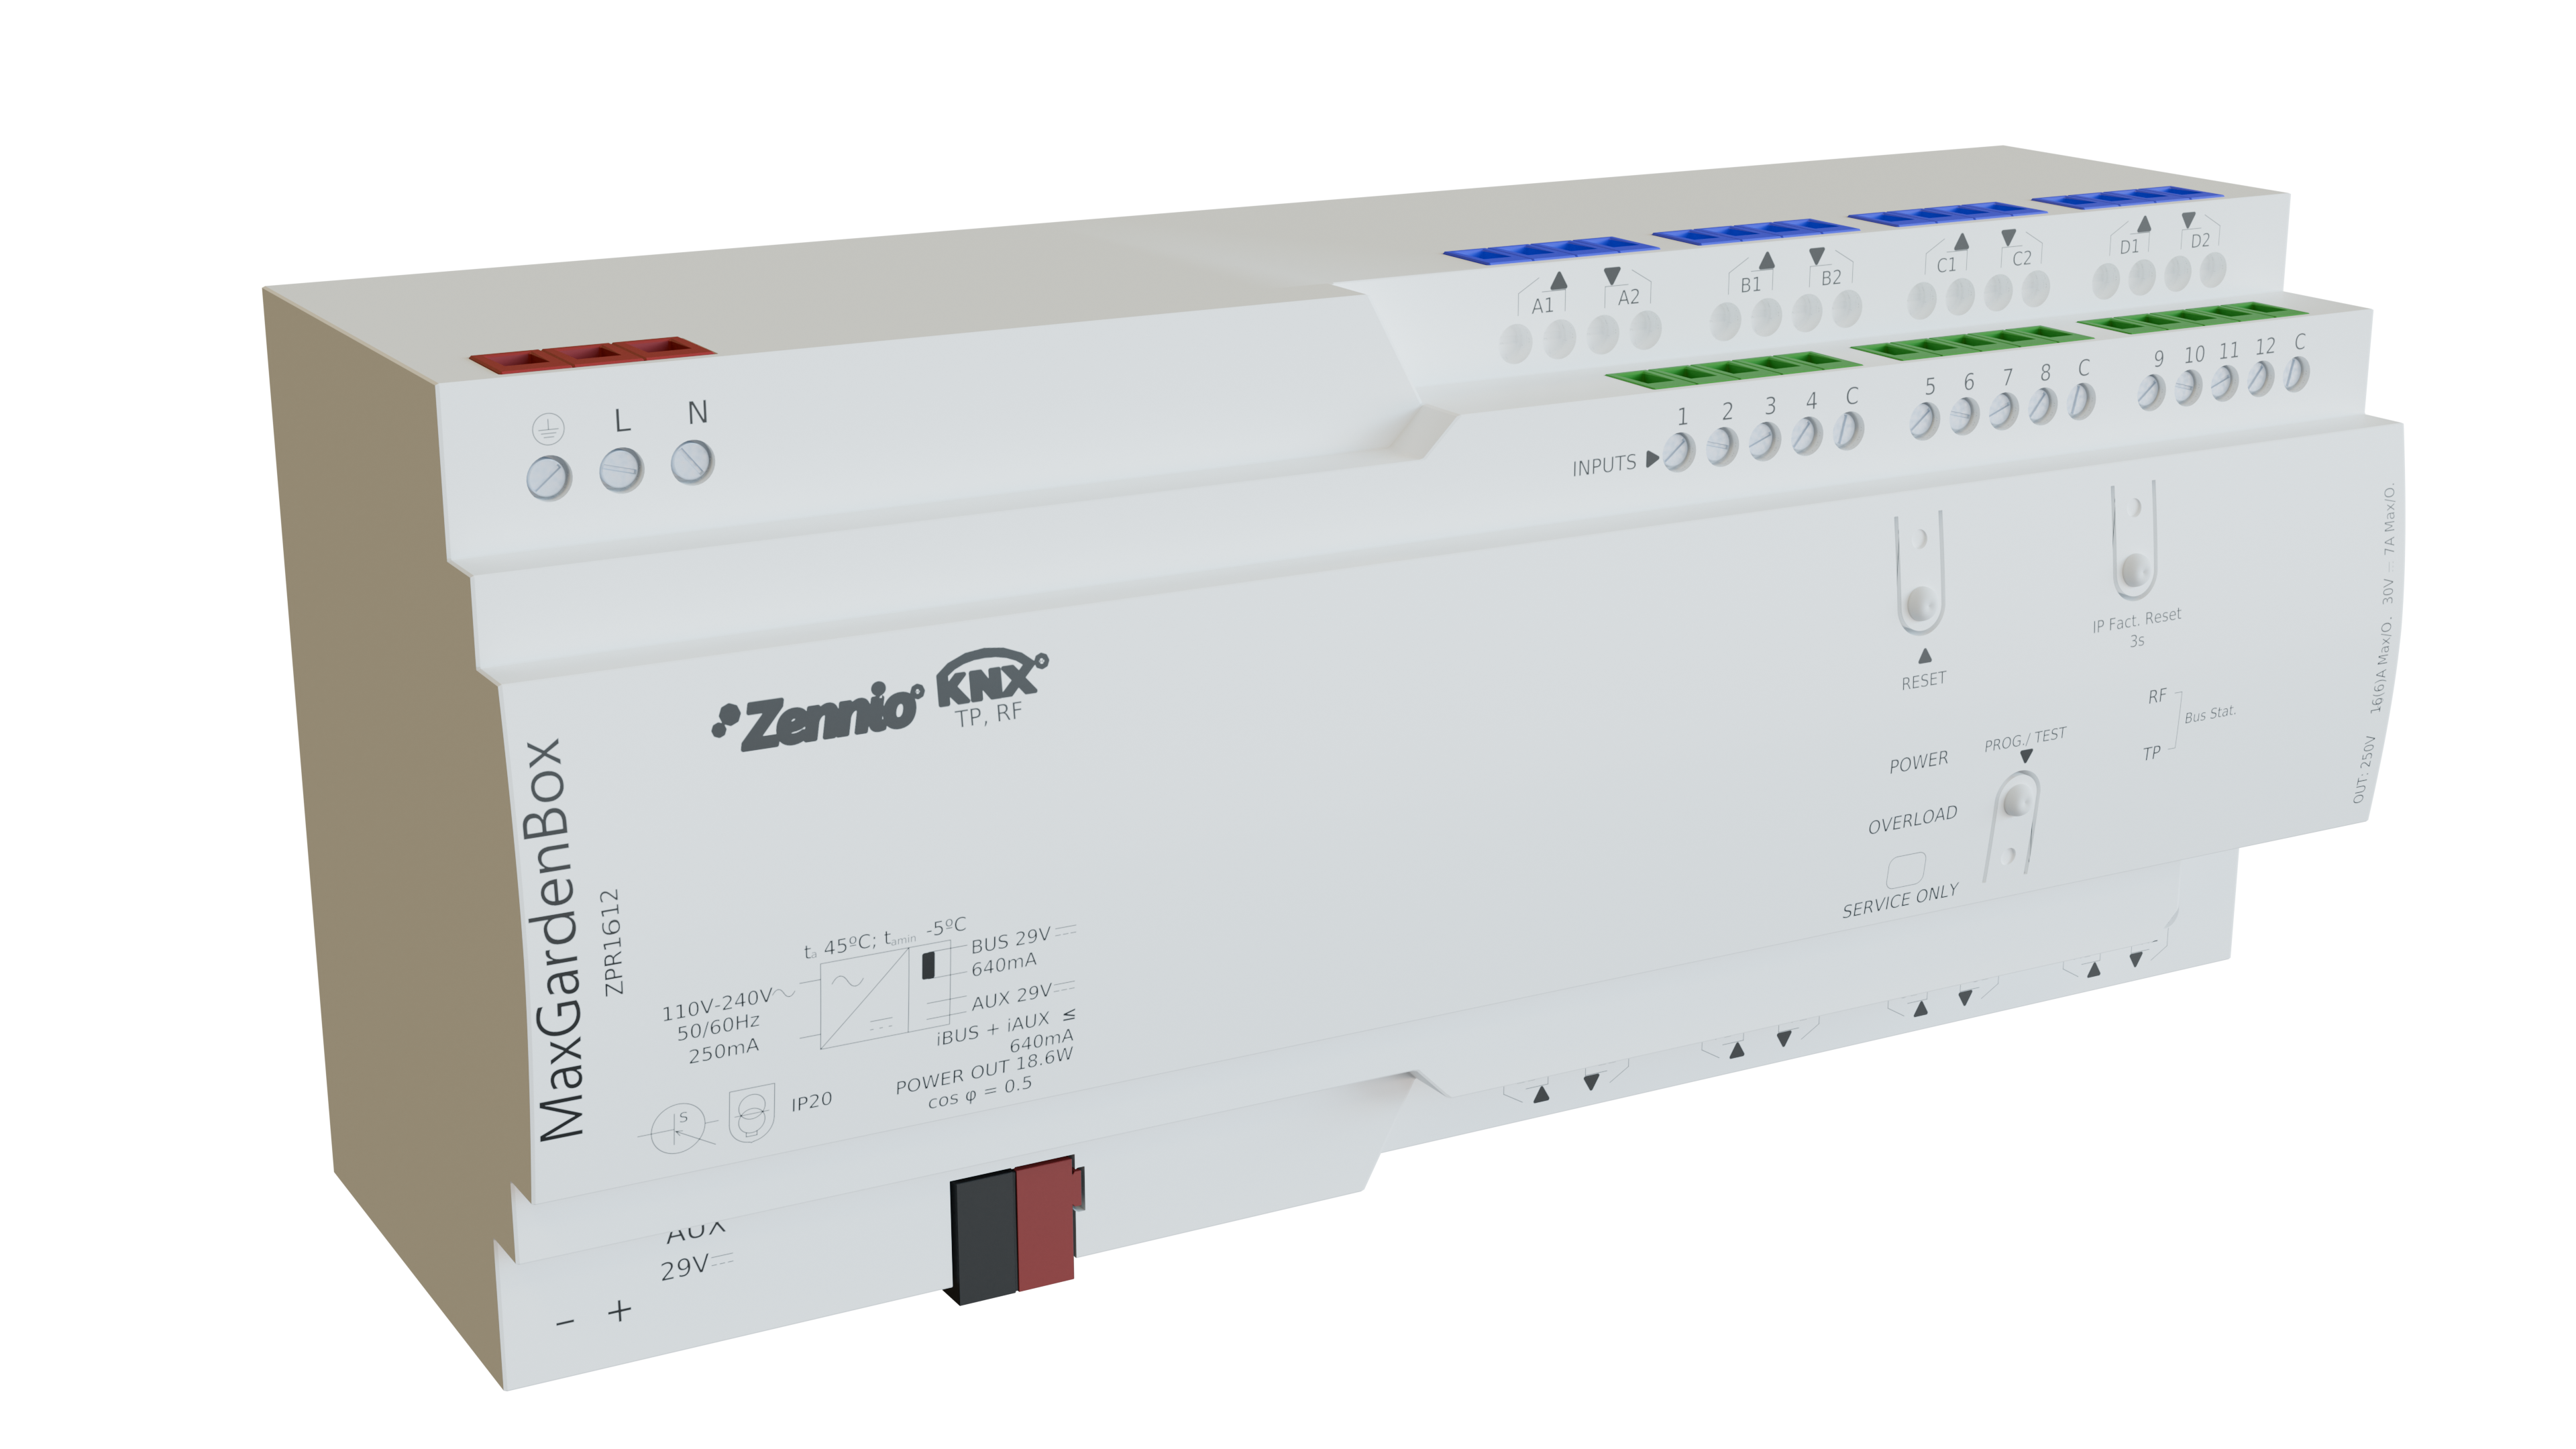
\includegraphics[width=0.5\linewidth]{fig/render2}
    \caption{MaxGardenBox}
    \label{fig:render2}
\end{figure}

El papel que finalmente se me asignó fue el de pruebas de integración, asegurar que el dispositivo funcione de forma correcta una vez sea instalado en un entorno real.

Para ello se empleó lo aprendido en \ref{sec:Pruebas y Testing}, organizándonos los encargados del testing de hardware y software, así como los desarrolladores del hardware.

El estudio de pruebas de integración se dividió en 3 fases principales:
\begin{enumerate}
    \item Descripción de la instalación
    \item Riegos y objetivos
    \item Ensayos
    \item Recursos necesarios
\end{enumerate}
    

\begin{figure}[h]
    \begin{subfigure}{0.5\textwidth}
        \includegraphics[width=0.9\linewidth]{"fig/Diagrama de integración"}
        \caption{Diagrama de integración}
        \label{fig:diagrama-de-integracion}
    \end{subfigure}
    \begin{subfigure}{0.5\textwidth}
        \includegraphics[width=0.9\linewidth]{"fig/Lista de ensayos"}
        \caption{Lista de ensayos}
        \label{table:lista-de-ensayos}
    \end{subfigure}5
\end{figure}

}
{

}


\section{Evaluación}
\label{sec:Evalucion}
A lo largo de todas las secciones se ha planteado una evaluación una vez finalizada esa formación. El estar siendo evaluado de forma semanal ayuda a incorporar los conceptos aprendidos, y sus correcciones facilitan reforzar los que no se hayan entendido.

Además, se ha realizado un examen que incorpora aspectos genéricos como resolución de problemas, cultura y ortografía, junto a todo lo aprendido a lo largo de la formación. El examen dura 4 horas y sirve tanto como para dar feedback al estudiante sobre cuanto ha aprendido como para que la empresa pueda valorar el rendimiento que el estudiante podría aportar a Zennio.
